\chapter{BGP state of the art}
\label{cha:bgp_art}

\ac{BGP} is the protocol used to control the information spreading on the Internet.
It is at the version \num{4} published in \num{2006} with the \ac{RFC} \num{4271}
\cite{rfc4271}.
\ac{BGP} is a \ac{PV} protocol, it distinguishes itself from the \ac{DV} and \ac{LS}
protocols with the major difference that it shares other than the knowledge of
a path also the path itself to reach the destination.

\ac{BGP} has two major sub-categories with a difference in the flow of information
direction:
\begin{itemize}
	\item \textbf{\textit{\ac{eBGP}}}, we talk about \ac{eBGP} when the
		flow of information goes from the inside
		of the \ac{AS} to other \acp{AS};
	\item \textbf{\textit{\ac{iBGP}}}, we talk about \ac{iBGP} when the flow
		of information goes from the outside of the \ac{AS} to the inside of
		it, to make aware of the new route also the internal routing protocol.
\end{itemize}

My main interest in this thesis is for the \ac{eBGP} part of the protocol, for
now on I will refer to it talking in general of \ac{BGP} without further distinguishing
from the internal protocol.

When there is an interconnection between two \acp{AS} that creates a \ac{BGP}
link, I will talk about peering referring to the connection, and those \ac{BGP}
speakers interconnected will be the peers.
Each \ac{BGP} link is based on a direct \ac{TCP} connection.
On these links, every \ac{AS} can configure its own policies that would be used
to evaluate routes at the reception or in the moment there is something new
to share.
There are three different possible type of relations that can be created by two
\ac{BGP} speaker, accordingly to the \ac{CAIDA}:

\begin{itemize}
	\item \textbf{\textit{\ac{c2p}}} This relationship highlights the fact that
		lower \ac{AS} pays a higher level \ac{AS} to get connectivity and access
		to the Internet;
	\item \textbf{\textit{\ac{p2p}}} This relationship is used to share the knowledge
		between two \acp{AS} of their customer providers without paying a higher
		level \ac{AS};
	\item \textbf{\textit{\ac{s2s}}} This relationship defines the connection
		between \acp{AS} under the same \ac{ISP}.
\end{itemize}

During this thesis, I will only consider the first two relationships \ac{c2p} and
\ac{p2p}, the schema in \Cref{fig:AS_flow} shows how the traffic is affected
based on the type of the link crossed.

\begin{figure}[ht]
    \centering
    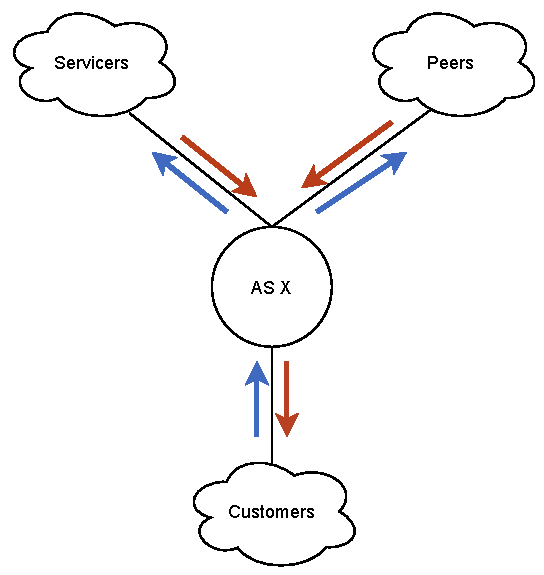
\includegraphics[scale=0.75]{images/BGP/ASKnowledgeDistribution.pdf}
	\caption{Distribution schema for the \acp{AS}, the row colours distinguish
	different flows, $AS\_X$ is a customer of the servicer set, a peer with the
	peers set and servicer for the customers set}
    \label{fig:AS_flow}
\end{figure}


As shown by the flows with a different colour in \Cref{fig:AS_flow} a single
\ac{AS} will share information considering the receiving link.
If something comes from one of its customers it will share the knowledge with
every other link that it has, even other customers (always respecting the output policies).
If a route has come from its provider or a peer then it will be only shared with
its own customers.
Those policies are commonly called \q{valley-free} and are dictated by convenience,
an \ac{AS} has all the advantages when
other \acp{AS} decide to use it to reach a specific destination.
For this reason is convinient for an \ac{AS} that everyone knows about its clients
networks, and, in the opposite side, that its clients knowes only the route
through it to reach other networks.

This behaviour can be modelled with a variant of the \ac{SSP} algebra described
in \cite{daggitt2018rate}.
This is the same algebra that will be used in \Cref{cha:des} to describe the links
relationships.

%\begin{itemize}
%    \item BGP de facto standard on the internet
%    \item What is an AS
%    \item interconnection between ASes
%\end{itemize}

\section{BGP}
\label{sec:bgp_intro}

Once a \ac{BGP} node has established a connection with another peer it will
start to exchange routes with that neighbour, always respecting the policies.
Its important to underline that, a \ac{BGP} speaker only shares its best routes
and in this protocol the best decision is dictated by the policies, and
then other possibilities would be evaluated (number of hops, bandwidth etc).
For this reason the best path decided by a node could differ from the actual
best path from a topological point of view.

Every \ac{BGP} node has a \ac{RIB} as data structure to keep the information
about the received routes, the alternative routes and what should be exported.
The \ac{RIB} is divided into \num{3} sections.
\begin{itemize}
	\item \textbf{\textit{ADJ-RIB\_in}} This \ac{RIB} contains all the routes
		that have been received by other \ac{AS} in order to be evaluated;
	\item \textbf{\textit{LOC-RIB}} This \ac{RIB} contains all the best routes
		that have been chosen from the \textit{ADJ-RIB\_in} from the node;
	\item \textbf{\textit{ADJ-RIB\_out}} There is an output \ac{RIB} for every
		neighbour of the node, it contains the route that should be advertised
		to the specific node.
\end{itemize}

One of the most important parts of \ac{BGP} is its decision process, that would
be applied to discern between the routes in the \textit{ADJ-RIB\_in} in order
to update the \textit{LOC-RIB} and, if necessary also the \textit{ADJ-RIB\_out}.
The decision process is composed of three parts:
\begin{itemize}
	\item[1] Calculation of the preference: This function is called every time
		there are new reachability information that needs to be evaluated, it
		will assign/update the preference value at every route in the
		\textit{ADJ-RIB\_in} using policy filters pre-configured. If a route
		doesn't respect the policy filters it will be then marked as ineligible,
		otherwise, a \textit{PREF\_VALUE} will be calculated and assigned to the
		route.
	\item[2] Route selection: This function is called at the end of the first
		phase, it collects all the eligible routes and evaluates them removing
		routes that would create loops or that creates conflicting situations.
		The evaluated routes are then ordered by the \textit{PREF\_VALUE} and
		then the best route will be then installed in the \textit{LOC-RIB}.
		In case of ties, there is an algorithm that can be used to break them.
	\item[3] Route dissemination: This function can be called in different
		situations, it will use the information in the \textit{LOC-RIB} to
		populate every \textit{ADJ-RIB\_out}, according to configuration
		policy.
\end{itemize}
The decision process is also responsible for the route aggregation and information
reduction.
At the end of the third phase, the \ac{BGP} speaker will execute the
\textit{Update-send} process, that is responsible for the effective dissemination.

There are multiple types of packets that can be sent by a \ac{BGP} speaker, but
we will focus only on the \ac{ADV} packets.
The \ac{ADV} packets are responsible for the dissemination of the information
to other nodes that will analyze and use the attribute inside the message
to assign a preference value to the route.
In particular, there are two sections of the \ac{ADV} messages that will
contain additive information and subtractive information.
We can distinguish \ac{ADV} messages using the type of information that are
transmitting:
\begin{itemize}
	\item \textbf{\textit{UPDATE}}, this type of messages represent the distribution
		of new reachability information, a new best route to a destination will be
		shared through an update message;
	\item \textbf{\textit{WITHDRAW}}, this type of messages are distributed when
		a node want to share that it doesn't know how to reach
		a destination anymore.
\end{itemize}
Inside those packets, there are different attributes that permit to transfer
information about the route (advertised or withdrawn).
There is an attribute that describes the address that the route represents,
another one that contains the path that will be used to reach the
destination, the next-hop used, etc.
During the years multiple new \ac{RFC} have introduced, modified, updated and removed
attributes that can be found inside an advertisement message.
Not all the attributes are mandatory for \ac{BGP} nodes, in fact, for a node
is possible to receive a route with an attribute that it is not able to interpret
but (if configured to do so) it will share the route with also the unknown
attributes.

Is important to remember that all those information are useful for the policy
filters that every node can have, for example, some nodes would automatically discard
any route that contains a specific \ac{AS} in the received path.

The \textit{Update-send} process is responsible for the distribution of the
messages that are stored in the \textit{ADJ-RIB\_out}.
It execute again some checks on the \ac{RIB}, removing unfeasible routes
and removing routes that have already been advertised to the pear.
It also has to respect a temporal constraint, introduced in \cite{rfc4271},
a \ac{BGP} speaker can't send to the same neighbour routes for the same destination
more often than the \ac{MRAI} value.
\ac{MRAI} act as a timer whose goal is to avoid continuous update storm caused
by decision changes in some peers in the network.

Another property that can be found in \ac{BGP} nodes that affects the messages
transmitted is the \ac{IW}.
This property permits to reduce the number of messages that are distributed.
Without this option when a \ac{BGP} node discovers a new best path to reach
a destination should send a withdraw followed by an update to its neighbourhood.
Thanks to this option is sufficient to send just the update, the other nodes
will learn that the best path is changed simply looking to the previous
alternative and comparing them.

%\begin{itemize}
%    \item High level of BGP
%    \item BGP messages
%    \item BGP Update messages
%    \item BGP policies
%	\item two type of BGP noise, the one caused by BGP itself and the one
%		caused by flapping interfaces
%\end{itemize}

%\section{BGP Wedgies}
%\label{sec:bgp_wedgies}
%
%\begin{itemize}
%    \item What are wedgies?
%    \item why are them important?
%    \item which situations them occur?
%\end{itemize}

\section{BGP inherent noise vs external noise}
\label{sec:bgp_noise}

With the term \textit{BGP Noise} I would like to define a particular behaviour
of \ac{BGP}.
It underline a situation where the nodes are distributing routes
that would be retrieved few moments later.
Producing an intense distribution of messages that are not optimal.
This behaviour is defined as noise because the tendency of \ac{BGP} to act
as echo-chamber and amplify this distribution of incorrect information.
%All those wrong messages are going to disturb the convergence of the protocol.
In fact, a \ac{BGP} node that receive an update for a neighbour will probably
redistribute the route to multiple neighbours, peers and servicer.
Given the hierarchical topology of the internet this behaviour grows
exponentially while the information reach the center of the network.

There are basically two sources of noises in \ac{BGP}, the inherent noise of
the protocol and the noise caused by external sources.
Those two type of noises are triggered by different causes and are
not discernible one another.

The first one is caused by the protocol itself when it tries to converge
on new knowledge.
The sharing of new routes can cause new \ac{ADV} that can then trigger the
\textit{Path Exploration} problem.
This is a noise caused by the protocol itself that acts as echo-chamber for
new best paths that change until the best possible path is taken in consideration.

One \ac{BGP} parameter tries to limit this noise acting as a message cache with
a compression system.
This parameter is \ac{MRAI} and it permits to avoid sending a message for every
new one received using a timer.
Only the best decision after that time will be shared.

The second type of noise is caused by a source outside the protocol.
A miss-configuration or a faulty interface can cause the send of not necessary messages.
For example, the withdraw and the advertisement of a route at a continuous interval.
This type of behaviour will cause continuous storms of messages and the triggering
of the first noise type.
Also, the transmission of a withdraw followed by an announcement is considered
a \q{flap}.

\ac{BGP} introduce a parameter with the \ac{RFC} \num{2439} \cite{rfc2439} that
is called \ac{RFD} to overcome this behaviour.
This parameter increases a value every time a flap or a route change are detected,
when this value passes a predefined threshold the route will be suppressed.
This value will always decay using an exponential decay function, even if it
doesn't overpass the threshold.
The decay function is calculated defining the time that the function should take
to half the value, by default \SI{15}{\minute}.
Once the route has been suppressed the \ac{BGP} speaker must wait enough time
that the value goes below another threshold before sharing it again.

Those two parameters are clearly connected one another from the fact that
one triggers the other and vice versa, is possible to create a particular topology
that has different performances based on the values assigned to those
parameters.
Think about two clique networks connected one another by only one node, that
node will act as a bottleneck, probably its \ac{RFD} threshold would be easily
overpassed and then it depends on its decay function before it can send
again the network to the second clique triggering \ac{MRAI} on those nodes that
will experience the path exploration problem.

%\fxfatal{I think that the graphs in Fig 2 and Fig 3 of Fabrikant et al. in
%\cite{fabrikant2011there} will easily trigger both \ac{MRAI} and \ac{RFD}}

\section{BGP MRAI, designed to reduce inherent noise}
\label{sec:bgp_mrai}

\ac{MRAI} is one of the parameters that mostly affect the convergence of \ac{BGP}.
A high value of it could unnecessarily delay the transmission of messages, but,
in the opposite case, a value too small can provoke a lot of messages, one for
every decision change of the node.
The main function of it is to reduce the intrinsic noise of \ac{BGP} compressing
the messages received.
There are a lot of studies about it, and it has already been shown that
the number of messages and the convergence time can depend on it \cite{griffin2001experimental}.
Also, it has been already proven by Fabrikant, Rexford et al. \cite{fabrikant2011there}
that an incorrect configuration of it could lead to tremendous consequences.

\ac{MRAI} has been introduced in the \num{4}Th version of \ac{BGP} \cite{rfc4271} and
it is nowadays a mandatory mechanism for every \ac{BGP} node, otherwise the load
in terms of messages to process and decision changes would be incalculable.
Its main purpose, as anticipated in \Cref{sec:bgp_noise} is to prevent, or
at least mitigate the noise created by \ac{BGP} itself.

At the base of \ac{MRAI}, there is a timer that controls how much time must pass
between one \ac{ADV} and the following one.
The timer is peer-based, for each interconnection an \ac{AS} could have a different
\ac{MRAI}, but it acts for every destination in parallel, this means that there
is a different timer for each destination that a node would share for every
\ac{BGP} relations that it has.
The idea behind it is that, in the period of time between one \ac{ADV} and the
following one the \ac{BGP} node will be able to receive other possible routes.
Being able to evaluate them and transmit a decision considering multiple alternatives.
It has the property to compress the input messages sequence in order to have
an output message sequence with a smaller number of \ac{ADV}.

The behaviour of a \ac{BGP} node with \ac{MRAI} is defined as follow for every
change in the \textit{ADJ-RIB\_out} of a neighbour caused by the
\textit{Update-send} process:
\begin{itemize}
	\item If there isn't an active \ac{MRAI} timer for the destination changed
		send the \ac{ADV} and set an \ac{MRAI} timer.
	\item If there is an active \ac{MRAI} timer for the destination then
		don't send anything.
	\item When the active \ac{MRAI} timer ends if there is still the necessity
		to send an \ac{ADV} then send it and set another \ac{MRAI} timer.
\end{itemize}

The second passage permits the route selection process to be executed multiple
times before the actual transmission of the decision.
That because \ac{MRAI} limits only the transmission and not the decision process.
The condition to the last passage is due to the fact that the compression some
times could lead to the not necessity to actually send a message.

The default value defined in the \ac{RFC} \num{4271} for \ac{MRAI} is equal to
\SI{30}{\second}.
But, \ac{MRAI} is a really controversial parameter, it has received multiple
revisions and studies.
In \num{2008} there has been a proposal to reset its default value to \SI{5}{\second}
\cite{jakma2008revised} thanks to different studies that take into consideration
the dimension of the topology and the latency \cite{qiu2005optimal}.
In \num{2010} a proposal \ac{RFC} of the \ac{IETF} \cite{jakma2010revisions}
says that the default would be left to the arbitrary choice of the operators and
that withdraw message could completely avoid it.
But this freedom would damage the convergence and the number of messages distributed
as showed by Fabrikant et al. \cite{fabrikant2011there}.

Is clear that \ac{MRAI} affect the network performances, but what affects \ac{MRAI}
and, by consequences, the performances?
Obviously, the choice itself of a different \ac{MRAI} strategy as showed for
example in \cite{milani2019BGP}, where the centrality has been used to obtain better
results in the case of network faults.
But, giving the fact that, the main function of \ac{MRAI} is to compress the
input messages also the sequence of messages receipt could be meaningful.
Giving that \ac{MRAI} is a link-based parameter also the number of links that
a node has could influence it and by consequences the position in the topology.
A well connected node will be more likely to receive multiple paths and messages
than one with only one link.

%\begin{itemize}
%    \item What is MRAI?
%	\item Rember that the MRAI purpose is to avoid the BGP noise
%    \item Previous works on MRAI
%    \item Suppositions on the MRAI influence
%\end{itemize}

\section{BGP RFD, designed to reduce external noise}
\label{sec:bgp_rfd}

\ac{RFD} is a parameter introduced in \ac{BGP} to overcome the problems caused
by the exterior sources of noise.
Its main function is to avoid fluctuating routes to overload \ac{BGP} nodes
with continuous message storms.
It has been introduced with the \ac{RFC} \num{2439} in \num{1998} \cite{rfc2439}.
Also, \ac{RFD} is a controversial parameter, it has been studied and evaluated again
different times, but, recent studies showed that the majority of the operators
still use deprecated values from \num{2001} \cite{gray2020bgp}.
Furthermore, other studies show that the majority of the \ac{ADV} that travels
through the Internet are generated by a restricted set of \acp{AS} but \ac{RFD}
seems to be too much restrictive and affect the majority of the \acp{AS} traffic
\cite{pelsser2011route}.

\ac{RFD} will use a single value, called \textit{figure of merit}, to evaluate
the actual situation of a route, while this value evolve the \ac{RFD} algorithm
will make a decision on what to do.
The evolution of the \textit{figure of merit} is dictated by the messages received,
with fluctuations, it will grow, while, over time, it will use a quadratic decay
function to decrease.
Fluctuations, or flaps, are represented by the reception of the withdraw and
the announcement of a route, a path change is also considered a flap, even
if thanks to \ac{IW} is limited to just one \ac{ADV}.

There are other parameters that are part of this \ac{BGP} component, the more
important are presented in \Cref{tbl:rfd_defaults}.

\begin{table}[ht]
	\begin{center}
	\begin{tabular}{ || m{5cm} | m{4cm} | m{4cm} || }
	\hline
			Parameter & Cisco default values & Juniper default values\\
	\hline \hline
			withdrawal penalty & 1.0 & 1.0 \\
	\hline
			re-advertisement penalty & 0.0 & 1.0 \\
	\hline
			attribute change penalty & 0.5 & 0.5 \\
	\hline
			suppress threshold & 2.0 & 3.0\\
	\hline
			half-life (min) & 15 (900s) & 15 (900s)\\
	\hline
			Reuse Threshold & 0.75 & 0.75 \\
	\hline
			Max Suppress Time (min.) & 60 (3600s) & 60 (3600s)\\
	\hline
	\end{tabular}
\end{center}

	\caption{\ac{RFD} parameters}
	\label{tbl:rfd_defaults}
\end{table}

Other than the name of the parameters, in \Cref{tbl:rfd_defaults} is showed also
the default value decided by Cisco.
The \ac{RFC} \num{2439} \cite{rfc2439} gives some guidelines on how to set those
values but the actual choice is left to the discretion of implementors.
The first three parameters, \textit{Withdraw, re-advertisement, attribute change}
represent the penalty applied to the \textit{figure of merit} when the homonym event
happen.
The \textit{suppression threshold} represents the level at which the \ac{BGP} node will
suppress the route and don't advertise it until the figure of merit goes
below the \textit{reuse threshold}.
The decay of the \textit{figure of merit} follows a quadratic decay function
which rate is calculated using the \textit{Half-life} parameter.
the \textit{Max Suppress Time} will override all this parameters because, as
defined in the original \ac{RFC}, a route cannot be suppressed for more than
that time, it doesn't matter the figure of merit accumulated by this route.

An example of the figure of merit evolution could be seen in \Cref{fig:figure_of_merit},
This image has been taken from \cite{gray2020bgp}.

\begin{figure}[ht]
    \centering
    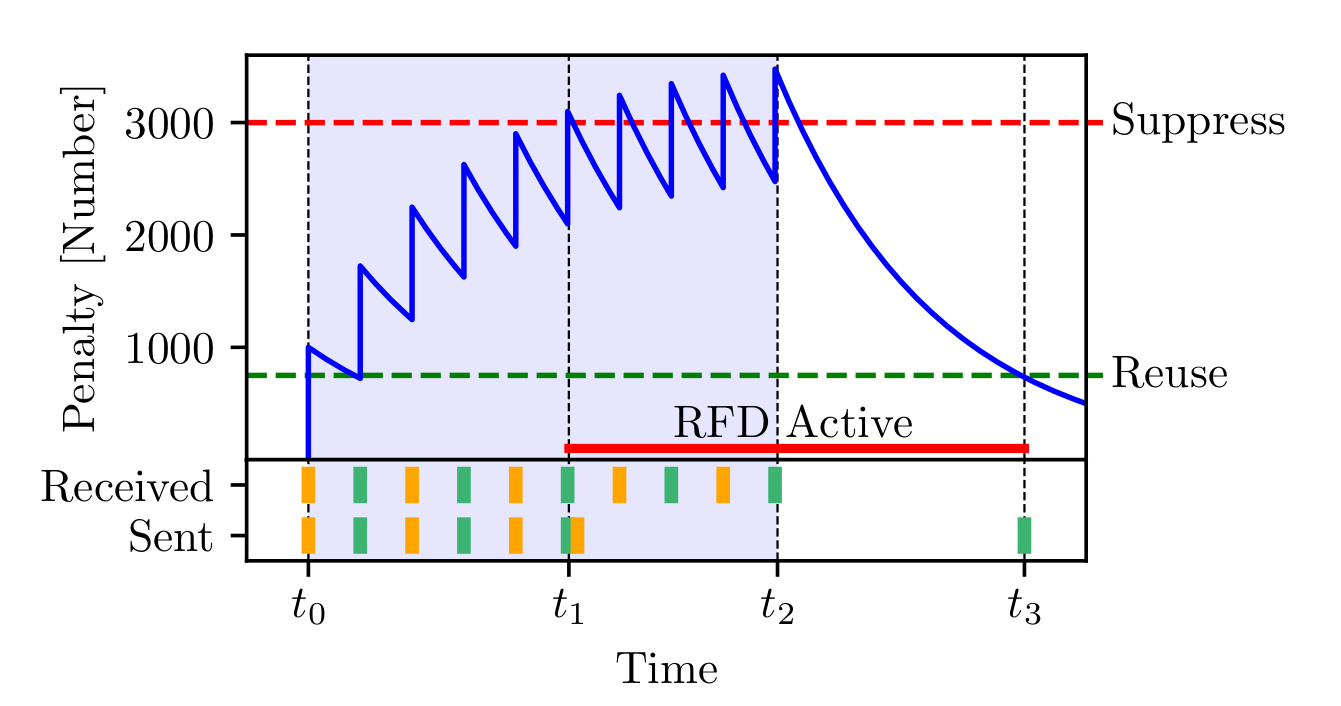
\includegraphics[scale=0.22]{images/RFD/evolution.png}
	\caption{Example of evolution of the \ac{RFD} \textit{figure of merit} taken
	from \cite{gray2020bgp}, yellow messages represent withdraws and green ones
	are advertisement, the dashed lines are the suppression and reuse threshold}
    \label{fig:figure_of_merit}
\end{figure}

\Cref{fig:figure_of_merit} shows a hypothetic evolution of the \ac{RFD} filter,
it doesn't rely on the default value of the Cisco implementation.
Is possible to see in the lower part of the plot the messages received by the
\ac{BGP} speaker, yellow one represent withdraws while the green are announcements.
Is possible to see that the penalty value grows at each flap and as soon it reaches
the suppression threshold the route will not be advertised to any neighbour.
While after the decay has reached the reuse level is possible to advertise the
route again.

Is possible to see that \ac{RFD} doesn't make any difference on its own on what
is causing the flaps, it simply reacts to the actual situation of the network.
Is not even possible to determine where is located the flap, if the source
is flapping heavily for some reasons or there is an \ac{AS} in the middle of the
path that is malfunctioning.

\ac{RFD} has a troubled history, maybe even more than \ac{MRAI}.
In \num{2006}, thanks to the publication of \cite{mao2002route}, the \ac{RIPE}
recommends to disable it\cite{smith2006ripe}.
A few years later the publication of the article from Pelsser et al. \cite{pelsser2011route}
\ac{RIPE} and \ac{IETF} shares that now \ac{RFD} should be used with the updated
parameters \cite{bush2013ripe,rfc7196}.
Unfortunately, the study from Gray et al. \cite{gray2020bgp} in \num{2020} shows
that the majority of the \ac{AS} uses \ac{RFD} with outdated parameters
from the \ac{RFC} \num{2439}.

\ac{RFD} can influence the network convergence time, and this behaviour is
mostly impacted by the threshold and the decay function applied to the figure
of metit.
A more permissive threshold could be helpful in situations where the flaps are
caused by transitional behaviour.
I will study and analyze the impact of the threshold in \Cref{cha:bgp_rfd}.

%\begin{itemize}
%    \item What is RFD?
%	\item Remember that RFD purpose is to avoid the noise produced
%		by route flapping
%	\item RFD cant distinguish the noise, is to restrictive, R bush point to
%		avoid the use of RFD for the first noise increasing the threshold.
%    \item Why is used RFD?
%    \item Evolution of RFD?
%    \item RFD Today
%\end{itemize}

\section{Topologies}
\label{sec:topologies}

%The study of the tomografy of the internet has been a really \q{hot} topic in the
%90's.
%Is not possible to know exactly the Internet network, thats because the edges
%of the network are defined by commercial contracts between the nodes that are
%kept private between the parts.
%
%We are not compleatly blind, we know some properities of the network.
%Internet is a hierarchical topology where there
%are different layers of nodes interconnected one anothere and different types of
%nodes.
%The nodes in the highest level, Tier one nodes, are the nodes that interconnect
%all the lower layers of the network and them are
%connected one another in a clique network.

\ac{BGP} has been designed to throw away information.
Is important to remember that the actual topology of the Internet depends on the
level of abstraction required.
If we consider the graph of the relationships within the \acp{AS} is not
possible to assume that this also represents the geographical graph.
In fact, one \ac{AS} can have multiple connections with another \ac{AS}
that are distributed along different geographical points.
Is also possible to have a connection through a tunnel that will permit to have
a connection that physically passes over other devices.
Is possible to see an example of this distinction in \Cref{fig:astopology_vs_internet}

\begin{figure}[ht]
     \centering
     \begin{subfigure}[b]{0.45\textwidth}
         \centering
         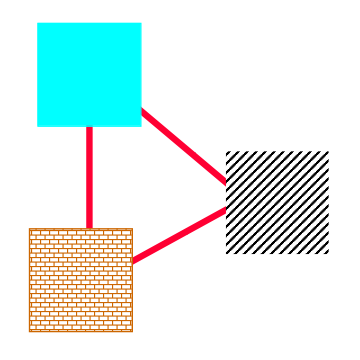
\includegraphics[width=\textwidth]{images/BGP/ASTopology.png}
		 \caption{\ac{AS} Graph}
         \label{fig:as_graph}
     \end{subfigure}
     \hfill
     \begin{subfigure}[b]{0.45\textwidth}
         \centering
         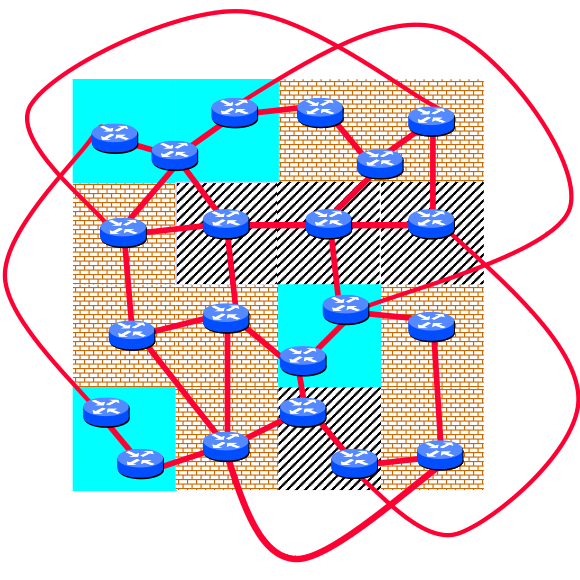
\includegraphics[width=\textwidth]{images/BGP/InternetTopology.png}
		 \caption{Actual geographical topology}
         \label{fig:actual_topology}
     \end{subfigure}
		\caption{Differences between two levels of detail on the Internet graph}
        \label{fig:astopology_vs_internet}
\end{figure}

In this thesis I will consider only the first case, all my topologies are composed by
the connections between the \acp{AS} without considering the actual physical layer
where this interconnection resides.

I will then use three different topologies to show particular situations or
behaviours of the network with certain events.
\begin{itemize}
	\item \textbf{\textit{Clique topology}}, This topology represent the higher
		level of the internet, in fact, all the Tier one nodes are interconnected
		in a clique network;
	\item \textbf{\textit{Fabrikant topology}}, This is a particular topology
		because it represent a special case that can be present in the internet,
		and also is possible to show that special configurations of this topology
		can lead to difficult situations.
	\item \textbf{\textit{Internet-like topology}}, This kind of topologies
		have the goal to resemble the real internet using statistical information
		about it.
\end{itemize}

I choose the clique topology because it is one of the possibly worst
case scenario for a \ac{BGP} network, accordingly with \cite{labovitz2000delayed}.
A clique graph could be composed by an $n$ number of nodes, and every node has
$n-1$ edges towards every other node.
An example of clique topology can be sawed in \cref{fig:clique_topology}, I added
two nodes to the network, outside the clique, in order to be able to have an
input and an output point.

The Fabrikant topology is inspired by \cite{fabrikant2011there} where is used
a similar chain network to show, in a theoretical way, how an uncontrolled
\ac{MRAI} setting could lead to explosive situations.
This topology will be used for the same purpose in this thesis, an example
of it is showed in \Cref{fig:fabrikant_topology}.
The explosion is caused by the \textit{Path exploration} problem, at a certain
point the node \num{2} would change idea on which path to follow to reach $d$
and all nodes will go through a transition state where they will
share their backup path.

\begin{figure}[ht]
     \centering
     \begin{subfigure}[b]{0.45\textwidth}
         \centering
		 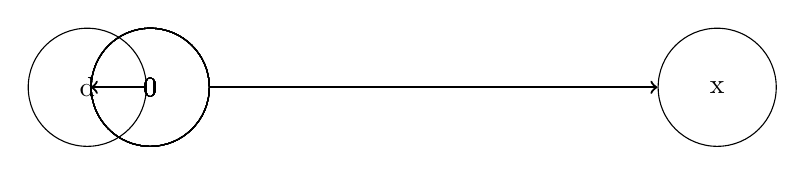
\begin{tikzpicture}[scale=0.2, every node/.style={draw=black,circle,inner sep=0pt}]
    \node [minimum size=1.5cm] (d) at (0,0) {d}; 
    \node [minimum size=1.5cm] (x) at (40,0) {x};                                    
    \node [minimum size=1.5cm] (0) at (4,0) {0};                                    
    \node [minimum size=1.5cm] (0) at (4,0) {0};                                    
    \node [minimum size=1.5cm] (0) at (4,0) {0};                                    
    \node [minimum size=1.5cm] (0) at (4,0) {0};                                    
    \node [minimum size=1.5cm] (0) at (4,0) {0};                                    
    \node [minimum size=1.5cm] (0) at (4,0) {0};                                    
    \node [minimum size=1.5cm] (0) at (4,0) {0};                                    
    \node [minimum size=1.5cm] (0) at (4,0) {0};                                    
    \node [minimum size=1.5cm] (0) at (4,0) {0};                                    
    \node [minimum size=1.5cm] (0) at (4,0) {0};                                    
    \draw [thick, ->] (d) -- (0);                                 
    \draw [thick, ->] (0) -- (x);                                 
\end{tikzpicture}                                                       
		 \caption{Clique graph example}
    	 \label{fig:clique_topology}
     \end{subfigure}
     \hfill
     \begin{subfigure}[b]{0.45\textwidth}
         \centering
         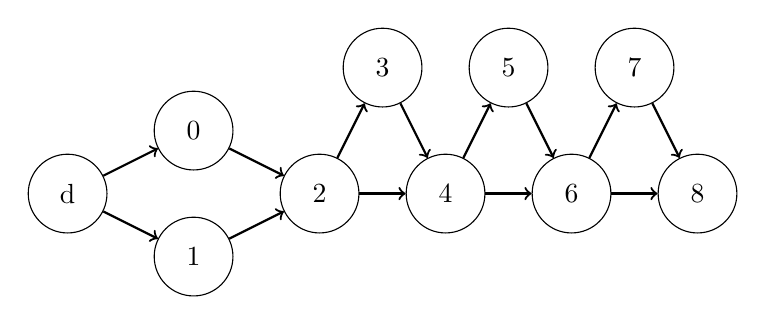
\begin{tikzpicture}[scale=0.2, every node/.style={draw=black,circle,inner sep=0pt}]
    \node [minimum size=1cm] (d) at (0,0) {d}; 
    \node [minimum size=1cm] (0) at (8,4) {0}; 
    \node [minimum size=1cm] (1) at (8,-4) {1}; 
    \node [minimum size=1cm] (2) at (16,0) {2}; 
    \node [minimum size=1cm] (3) at (20,8) {3}; 
    \node [minimum size=1cm] (4) at (24,0) {4}; 
    \node [minimum size=1cm] (5) at (28,8) {5}; 
    \node [minimum size=1cm] (6) at (32,0) {6}; 
    \node [minimum size=1cm] (7) at (36,8) {7}; 
    \node [minimum size=1cm] (8) at (40,0) {8}; 
    \draw [thick, ->] (d) -- (0);
    \draw [thick, ->] (d) -- (1);
    \draw [thick, ->] (0) -- (2);
    \draw [thick, ->] (1) -- (2);
    \draw [thick, ->] (2) -- (3);
    \draw [thick, ->] (2) -- (4);
    \draw [thick, ->] (3) -- (4);
    \draw [thick, ->] (4) -- (5);
    \draw [thick, ->] (4) -- (6);
    \draw [thick, ->] (5) -- (6);
    \draw [thick, ->] (6) -- (7);
    \draw [thick, ->] (6) -- (8);
    \draw [thick, ->] (7) -- (8);
\end{tikzpicture}                                                       


		 \caption{Fabrikant chain graph example}
		 \label{fig:fabrikant_topology}
     \end{subfigure}
		\caption{Simple topologies used in the thesis}
        \label{fig:clique_and_fabrikant}
\end{figure}

The last type of topology used points to resemble the properties of the actual
Internet graph.
It uses the property studied and described by Elmokashfi et al. in \cite{elmokashfi2010scalability}.
An example with few nodes is available in \cref{fig:internet_like_topology}.
The internet graph is actually a hierarchical graph clearly separated in different
levels by the type and properties of the nodes.

\begin{figure}[ht]
     \centering
     \begin{subfigure}[b]{0.4\textwidth}
         \centering
         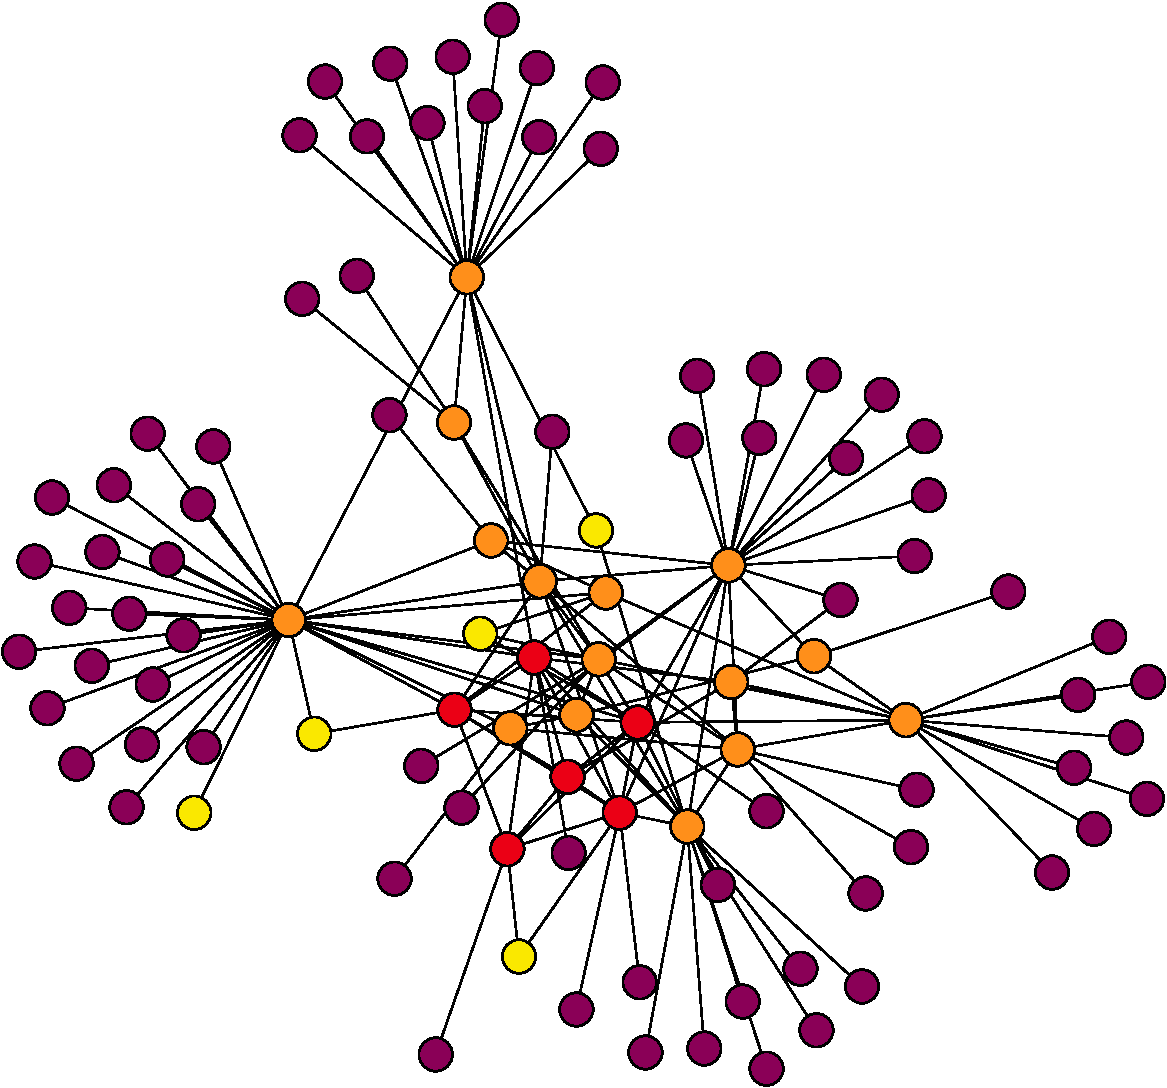
\includegraphics[width=\textwidth]{images/internet_graph/graph-100-colored.pdf}
		 \caption{Internet like graph with an \q{explosive}}
         \label{fig:internet_topology_explosive}
     \end{subfigure}
     \hfill
     \begin{subfigure}[b]{0.4\textwidth}
         \centering
         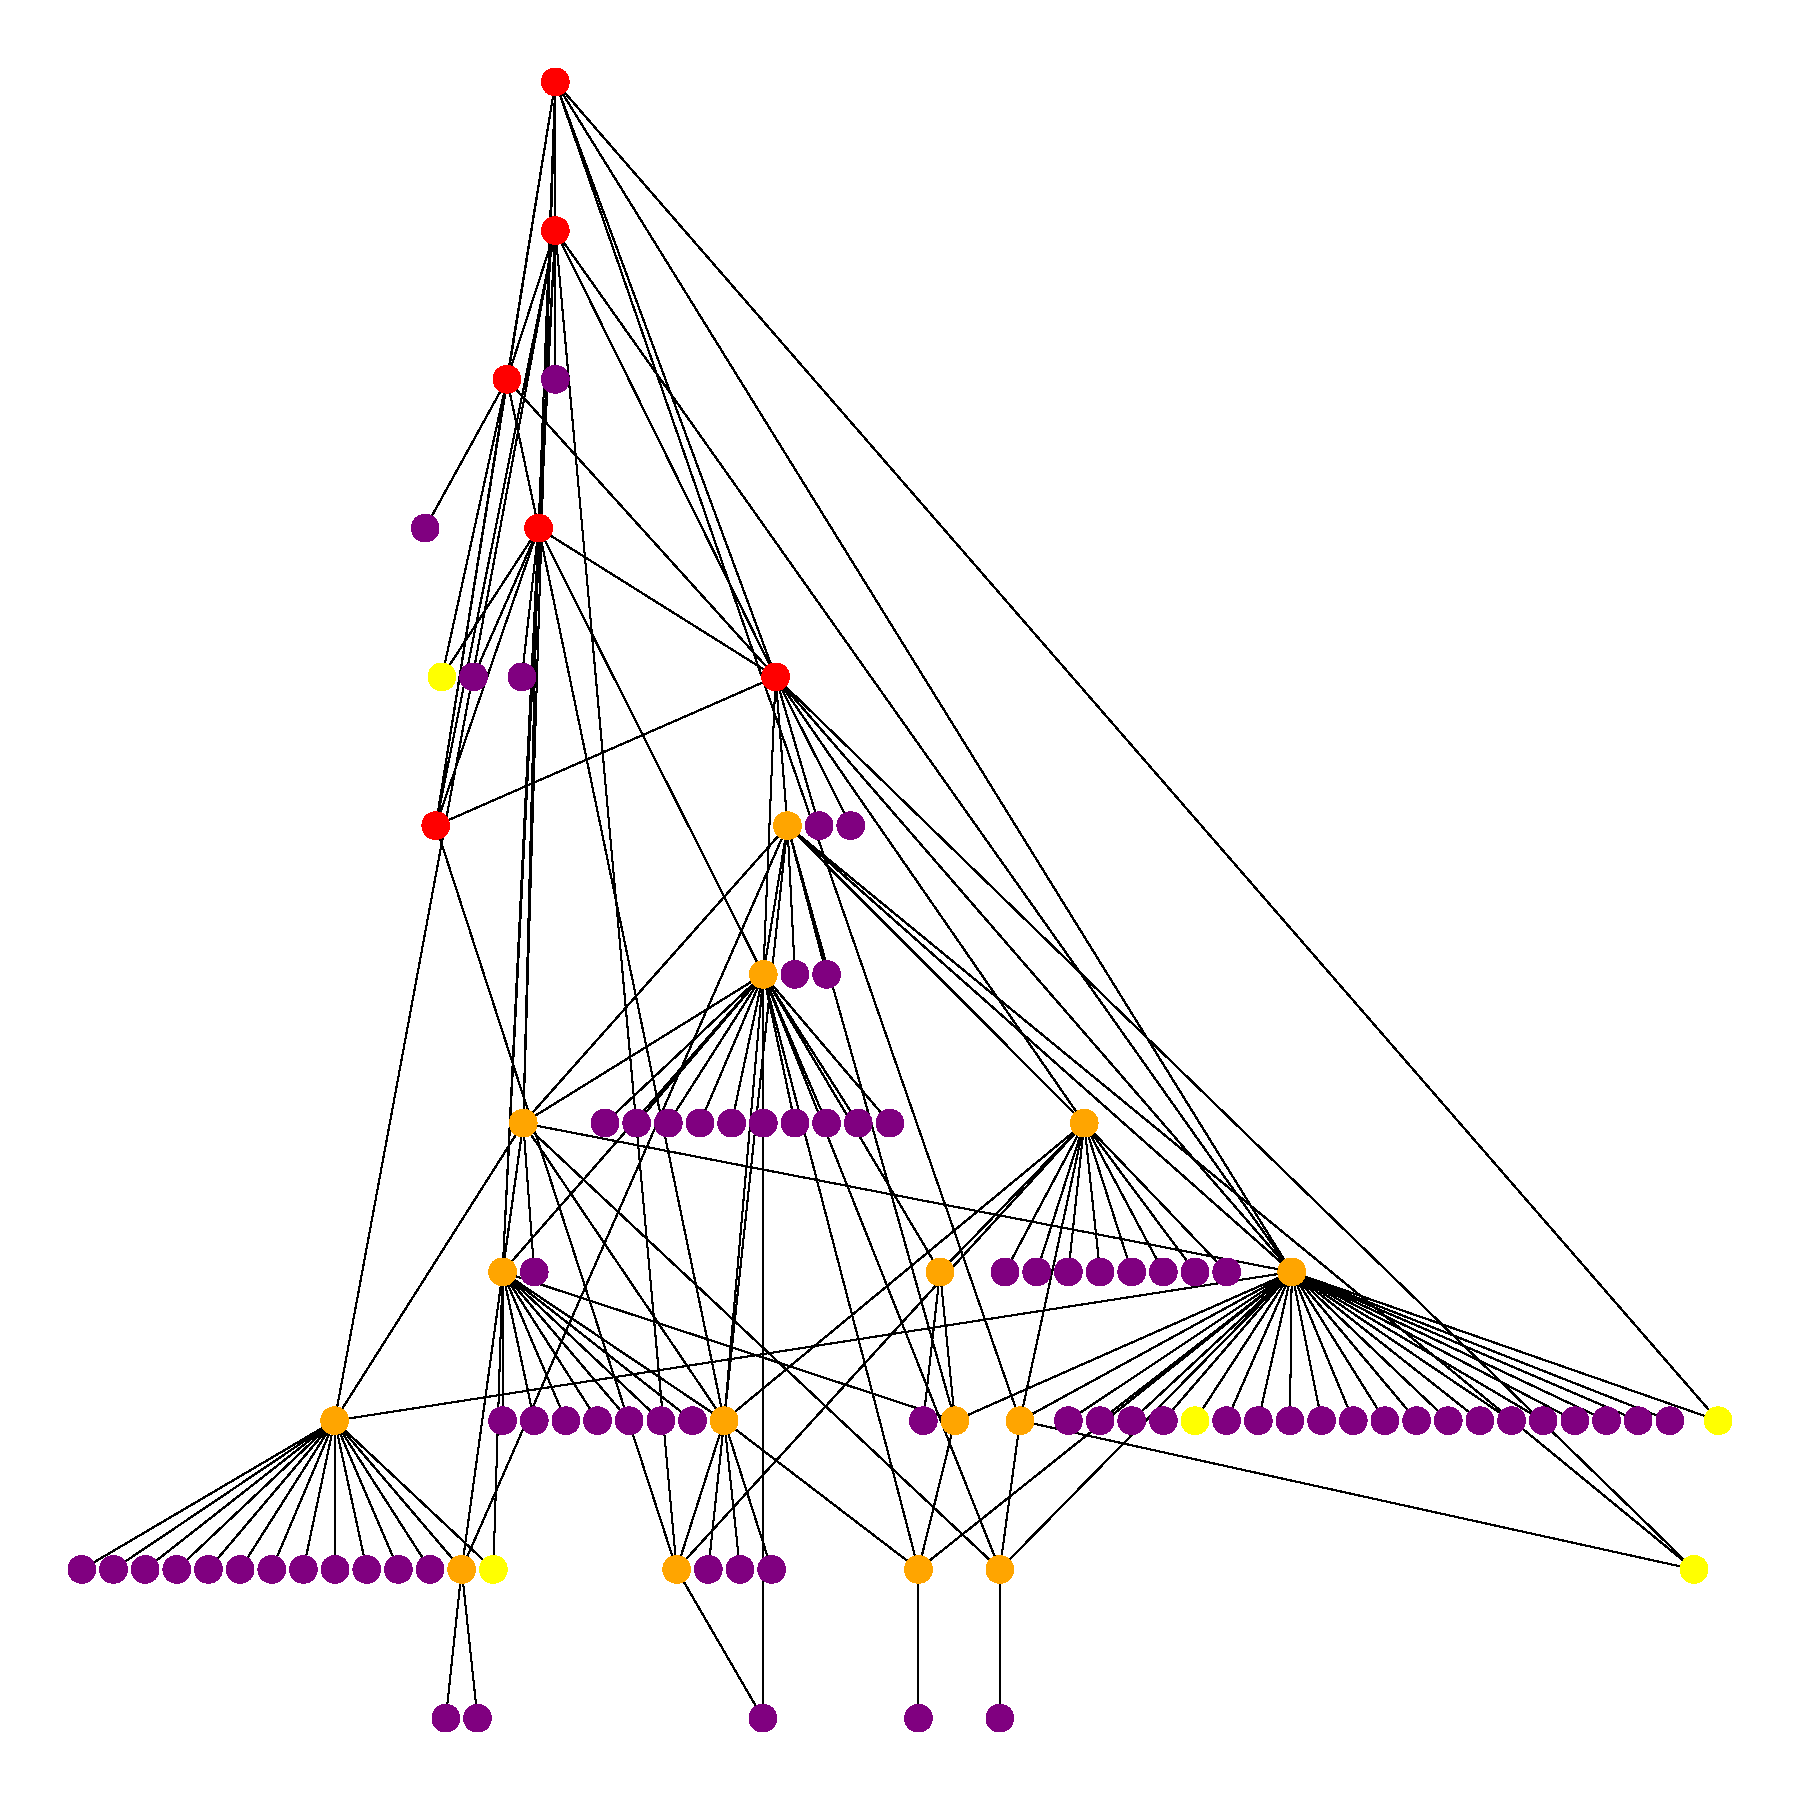
\includegraphics[width=\textwidth]{images/internet_graph/graph_dot.pdf}
		 \caption{\q{Hierarchical} Internet like graph}
         \label{fig:internet_topology_hierarchical}
     \end{subfigure}
        \caption{Internet like graph coloured to show the hierarchical structure,
4 types of nodes, T (tier 1 mesh), M, CP, C (Customers, the purple one)}
        \label{fig:internet_like_topology}
\end{figure}
